\section{Evaluation}
\subsection{Methodology}
We experimentally evaluate FlexLION implementing the rack-level interconnect from the previous section and compare it to the discussed tree-based topologies. We stick to the same network configuration from Table~\ref{tab:properties} and Figure~\ref{fig:networktopologies} for all the networks and thus study the interconnect of a 256-node network. We use gem5~\cite{binkert2011gem5} with Garnet2.0~\cite{agarwal2009garnet} for detailed performance simulation. We evaluate the network under a range of traditional synthetic traffic patterns (uniform random, bit complement, tornado, shuffle) to stress all corner cases of the topologies. \\
To compare FlexLION with the most aggressive baseline, we model the power consumption and latency of the switches based on state-of-the-art commercially-available data center switches, which consume 95W power and offer a 100ns switch traversal latency~\cite{intelomnipath}~\cite{mellanox}. We consider two transceiver technologies in our study: 1) Intel's SiPh transceivers which consume 35pJ/bit with 100G line rate~\cite{intelsip} and represent the most advanced commercially-available technology, and 2) tightly-integrated electronic-photonic co-designed transceivers have been demonstrated at the research level that can consume as little as 2pJ/bit in a 65nm technology~\cite{li201525}\footnote{Technology-scaling with SPICE models show 0.55pJ/bit at 14nm.}. Table~\ref{fig:sipparameter} lists the parameters we used for power modeling of the SiPh components(transceivers and FlexLION). While we model our FlexLION only with SiPh transceivers 2), we model the legacy fat tree topologies with both transceiver types 1) and 2). These comparisons allow to reveal the power savings of FlexLION in comparison to legacy topologies with the same transceiver technology and to illustrate the total power saving potential that FlexLION provides compared to state-of-the-art topologies (i.e., fat trees) with the best commercially-available transceivers. 
\begin{table}[]
\centering
\caption{SiP Technology Parameters}
\label{fig:sipparameter}
\begin{tabular}{@{}lllll@{}}
\toprule
Parameter            & Value     & Parameter      & Value  &  \\ \midrule
Laser Efficiency     & 14\%      & Coupler Loss   & 1 dB   &  \\
Waveguide Loss       & 2.2 dB/cm & Photodiode     & 0.1 dB &  \\
Receiver Sensitivity & -17.7 dBm & Modulator Loss & 1 dB   &  \\
Add-drop Filter Loss & 1.5 dB    & Power Margin   & 3 dB   &  \\ \bottomrule
\end{tabular}
\end{table}
We study FlexLION with different degrees of reconfigurability to expose the benefits and drawbacks of providing different levels of flexibility (i.e., as discussed earlier, number of MRRs vs.\ performance gains): \textit{FlexLION\_Full} denotes full reconfigurability (i.e., each wavelength available to a sender can be re-assigned to any desired destinations), \textit{FlexLION\_Half} denotes half of the wavelengths can be re-assigned, and \textit{FlexLION\_Quarter} denotes a quarter of the wavelengths can be re-assigned. In addition, to study the impact reconfiguration can have, we include a simple all-to-all network without reconfiguration capability into our study (LION\_NoReconf). We modelled network configuration by analyzing the link utilizations in the network for each traffic pattern and subsequently assigned link bandwidth based on the utilization rate of the previous run. \\
We also study the trade-offs of the different SiPh color-blind switches inside FlexLION, i.e., MEMS, MZI, and MRR, with respect to power consumption. Note that, as discussed in the previous sections, the reconfiguration time of these technologies is similar and has low significance to the overall reconfiguration of the networks. Once reconfiguration is completed, there are virtually no latency differences between them either. Therefore, we only analyze their differences in power consumption.

\subsection{Performance Results}
Figure~\ref{fig:latsyn} shows the performance results for the different synthetic traffic patterns for varied offered network load. 
\begin{figure*}[t!]
        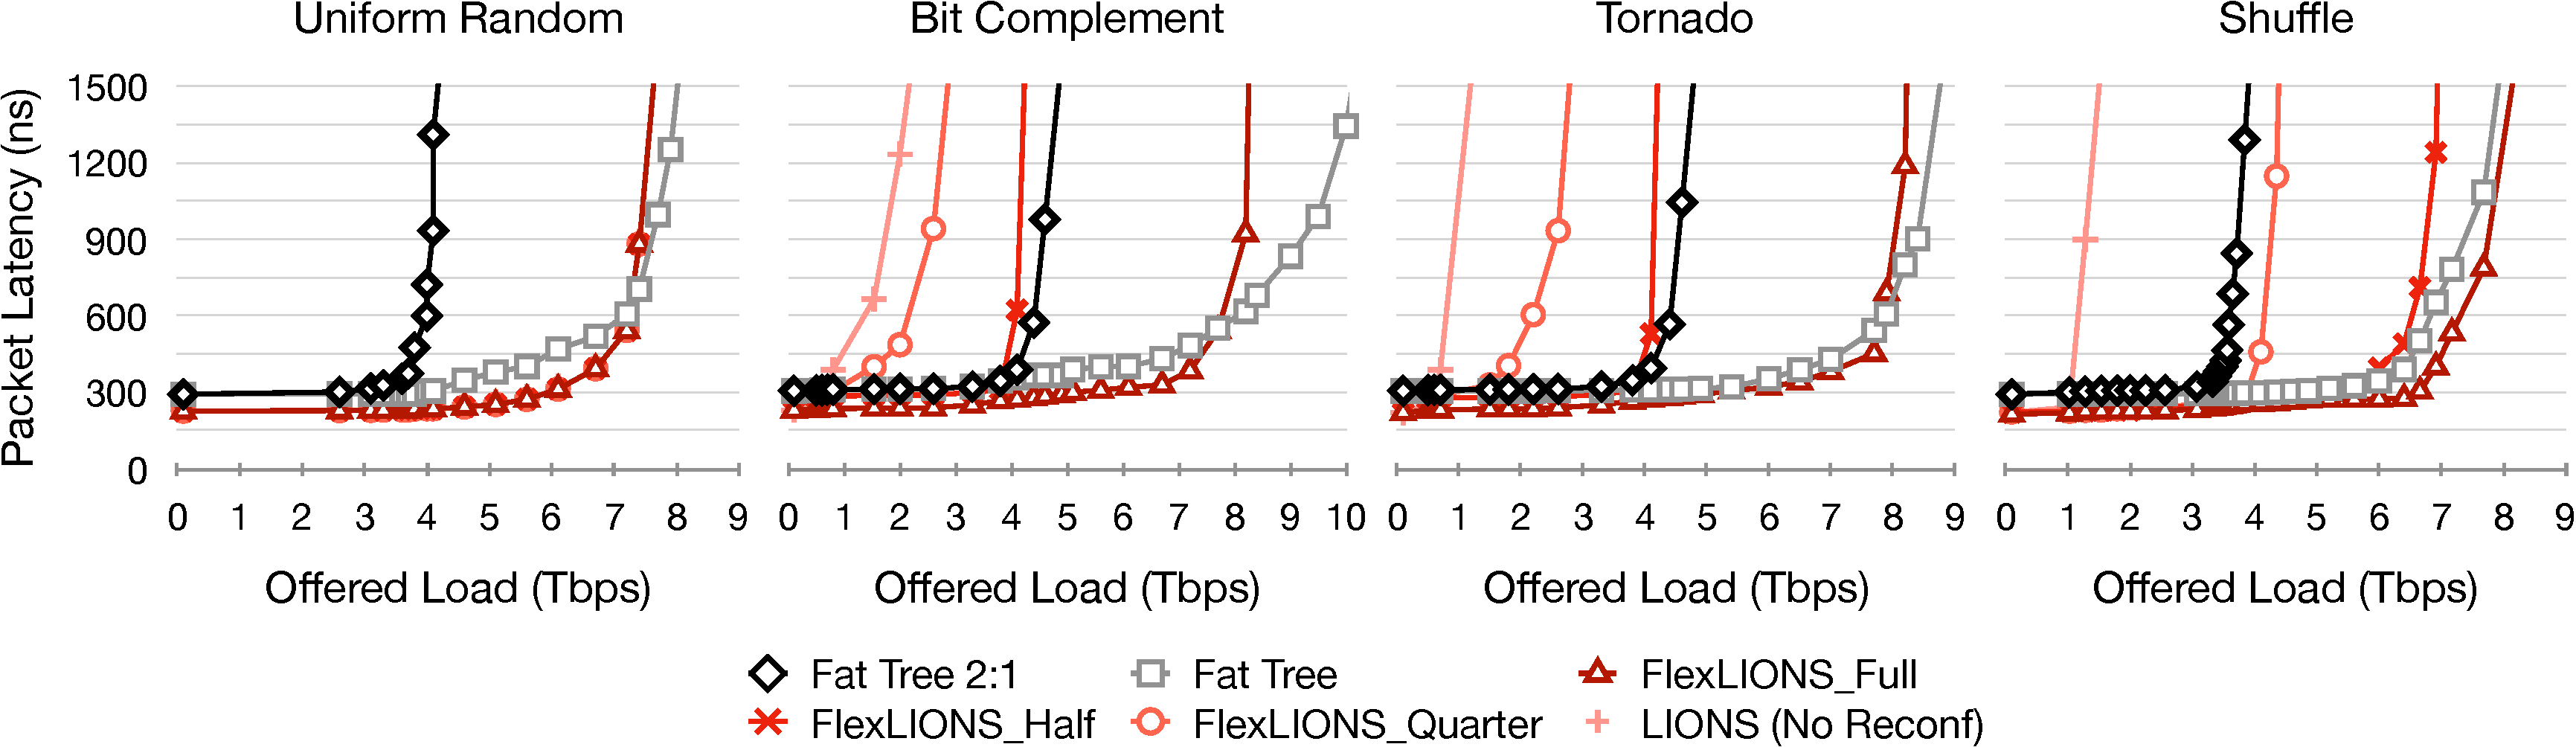
\includegraphics[width=\textwidth, clip]{Figures/syn.pdf}
        \caption{Average packet latency (ns) vs.\ offered load (Tbps) for different synthetic traffic patterns}
        		\label{fig:latsyn}
\end{figure*}
Given that the routing algorithms always choose the shortest path and that there is only one shortest path in an all-to-all network, LION without network configuration performs poorly for each traffic pattern aside from uniform random where traffic is evenly distributed across all links. Flexibility in bandwidth reconfiguration is therefore key if the traffic does not follow this corner case. For the different FlexLION reconfiguration capabilities, we observe that the more flexibility in the bandwidth assignment is available, the higher the total accepted traffic gets, which is in line with our hypothesis that fine-adjusting the bandwidth to links based on link utilization results in performance gains. \\
Compared to Fat Tree, which offers the same bisection bandwidth as FlexLIONS, FlexLION reduces the average packet latency prior to network saturation by 25\% on average which can be attributed to the lower average number of hops in FlexLION. FlexLION can compete with Fat Tree in terms of maximum throughput if it has full flexibility in terms of  wavelength reconfiguration for most traffic patterns. Compared to Fat Tree 2:1--a more light-weight implementation of the full Fat Tree--FlexLION nearly doubles the total bandwidth, and can compete even for lower levels of reconfiguration. 

\subsection{Power Results}
\subsubsection{Energy-per-bit}
Figure~\ref{fig:epb} illustrates the energy-per-bit (EPB) of the considered networks and transceiver technologies. Energy was calculated based on a FlexLION switch enabling full bandwidth reconfigurability (i.e. each wavelength can be assigned to any output port). LION indicates a full-mesh without bandwidth reconfiguration capabilities where the bandwidth is evenly distributed over all output ports. 
\begin{figure}[t!]
    \centering
        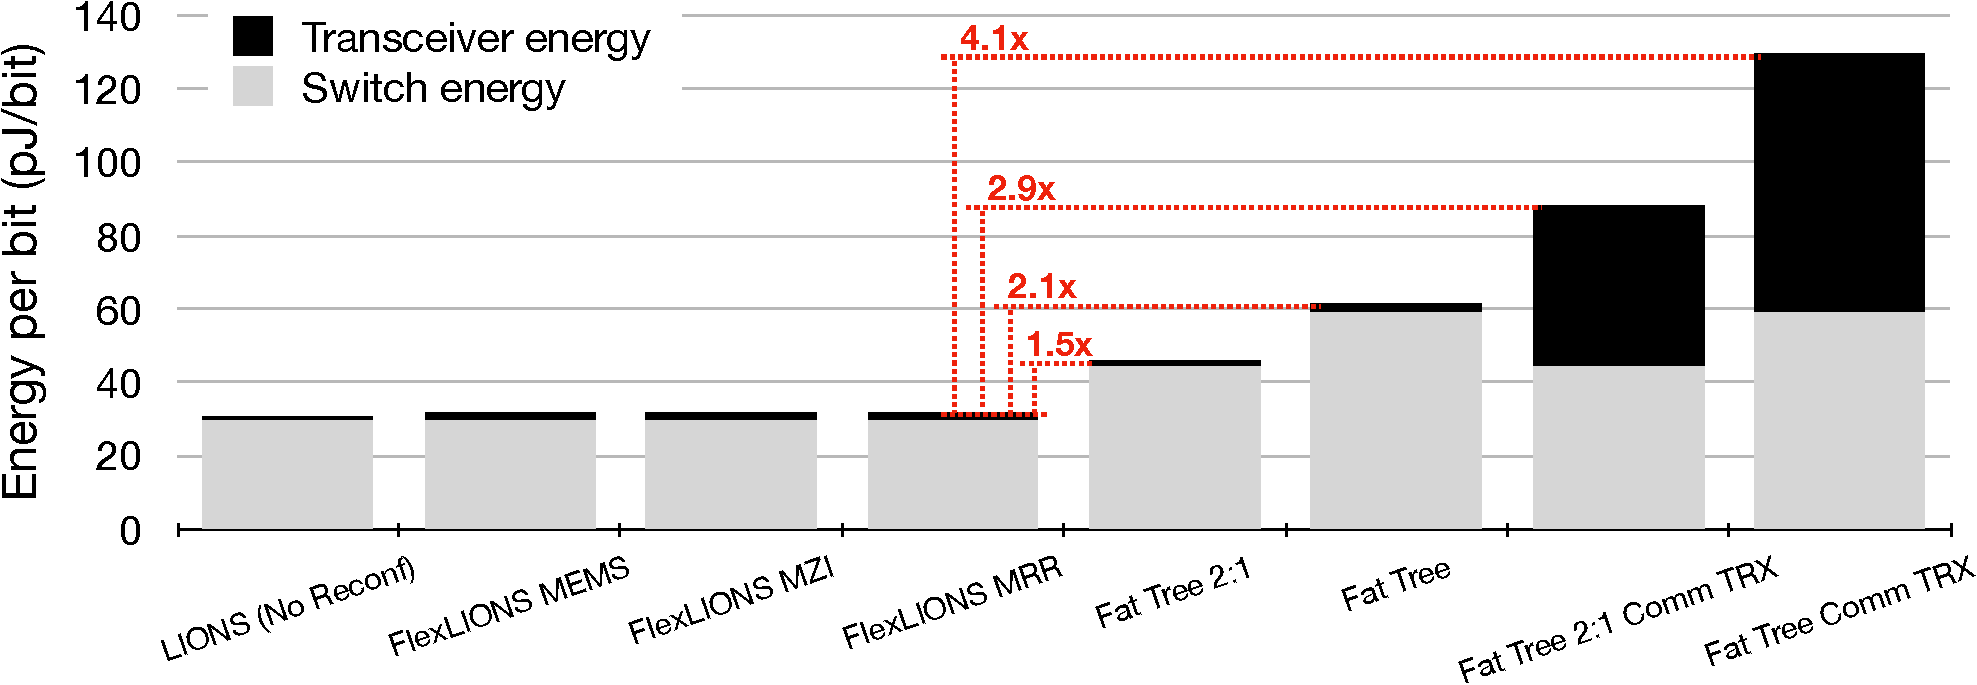
\includegraphics[width=\linewidth, clip]{Figures/epb.pdf}
    \caption[]{Energy-per-bit (pJ/bit) broken down into transceiver and switch energy of the different networks. `Comm' indicates commercially-available transceivers (TRX).}
    \label{fig:epb}
\end{figure}
The first observation is that the total energy is dominated by the network switches if the electronic-photonic co-designed transceivers are used. In this case, the reductions in power consumption between FlexLION and the fat tree topologies (2.1x (fat tree) and 1.5x (fat tree 2:1)) mostly comes from the energy saved by requiring fewer switches in the topology. \\
Depending on the color-blind switched used, FlexLIONS incurs higher losses and, in turn, higher power consumption. From a theoretical point of view, MEMS incurs the lowest loss of all color-blind switches (0.63dB vs. 2.16dB (MZI) and 2dB (MRR)); however, the high energy efficiency of the transceivers makes the energy differences of the different FlexLION designs negligible in the context of the whole network. The same applies to the degree of reconfiguration capability: the larger number of MRRs necessary to provide higher degree of flexibility cause higher path losses and higher power thermo-optical control of MRRs, but those impose negligible power overheads in a HPC network scenario, making FlexLIONS with full reconfigurability always the best design choice. \\
Compared to fat tree topologies with commercially-available transceivers, FlexLION offers up to 4.1x power reduction indicating the big impact that FlexLION could have compared to legacy designs. 

\subsubsection{Throughput-per-Watt}
Figure~\ref{fig:tpw} illustrates the TPW (maximum sustained throughput divided by power consumption) for the different network designs. Note that the power consumption for FlexLION's TPW values is based on a MEMS implementation (we omit the MZI and MRR based designs for simplicity as the difference in power consumption is $<$1\% and has a negligible impact on TPW). 
\begin{figure}[t!]
    \centering
        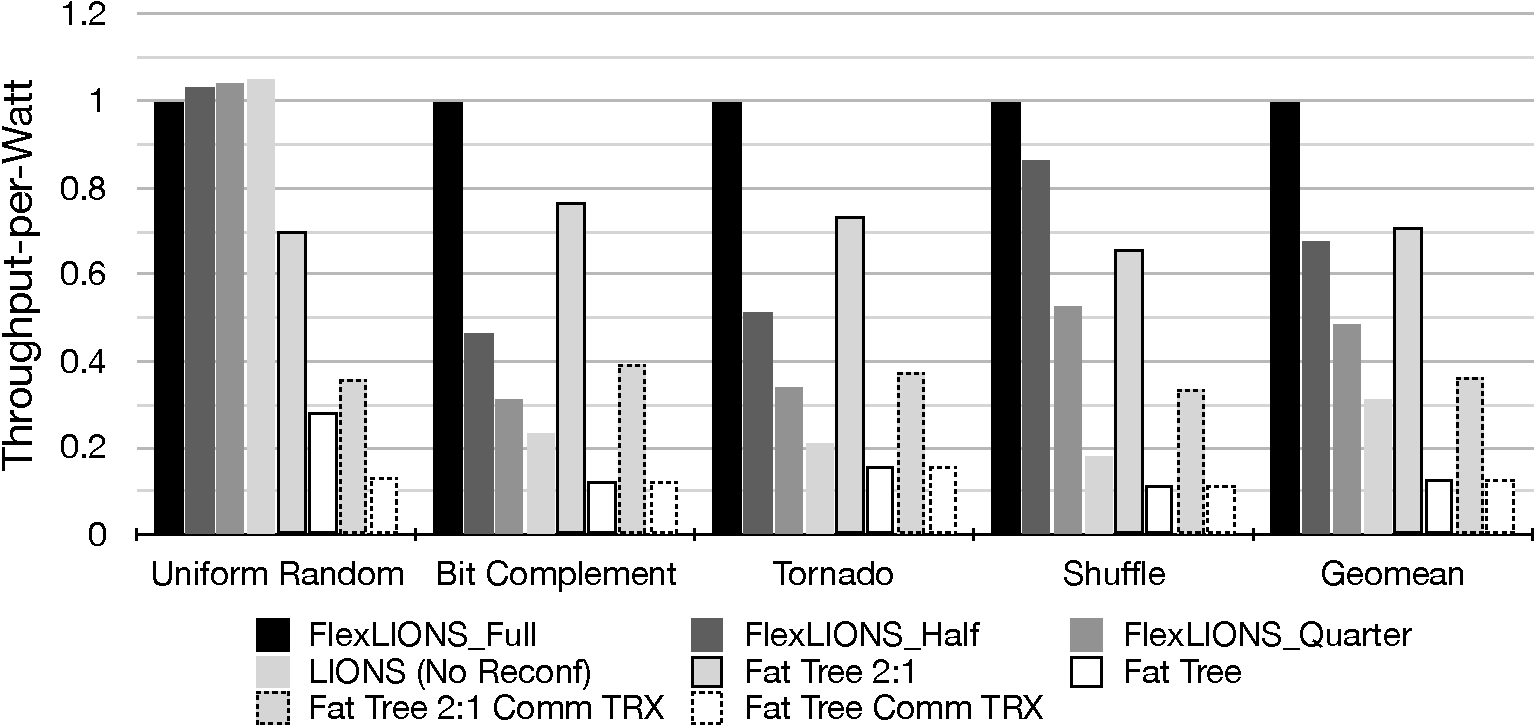
\includegraphics[width=\linewidth, clip]{Figures/tpw.pdf}
    \caption[Throughput-per-Watt (measured with maximum sustained throughput divided by power consumption) for the  different network designs normalized to FlexLION.]{Throughput-per-Watt (measured with maximum sustained throughput divided by power consumption) for the  different network designs normalized to FlexLIONS.}
    \label{fig:tpw}
\end{figure}
FlexLION outperforms all other designs significant on all traffic patterns. Fat tree 2:1 is the closest competitor but only exhibits 0.7x of FlexLIONS's TPW. Though supporting much less maximum throughput, Fat Tree 2:1 is actually more power efficient than a full Fat Tree as it saves a lot of power through exhibiting fewer switches and transceivers. In fact, our TPW results reveal that Fat Tree 2:1 would actually be more power efficient than FlexLIONS with reduced bandwidth reconfiguration capability, which waste much of their bandwidth on barely-utilized links. The network bandwidth reconfigurability of FlexLION is thus not only beneficial in terms of power efficiency, but also necessary to compete with state-of-the-art HPC networks. \\
In fact, unless traffic is perfectly uniformly distributed (in which case FlexLION without reconfigurability capability is the most power efficient as it provides the same throughput at reduced power), power efficiency in FlexLION is always the best with maximum flexibility in reconfiguration. However, such traffic patterns are very uncommon in HPC networks and are therefore of low practical relevance. 

\subsection{Discussion}
FlexLION interconnection fabric allows for all-to-all connectivity and full, fine-grained bandwidth reconfigurability from each input to each output port while successfully supporting line rates of 100Gb/s (as in legacy HPC interconnects). This fabric allows to significantly reduce the number of electronic switches and transceivers in HPC networks while providing similar maximum throughput at lower latency. While Fat Trees--the de-facto standard for HPC networks--offer a scalable fabric and load balancing, their resource requirements and higher network diameter make them inferior to FlexLIONS. \\
Effectively, FlexLION tightly-integrated and bandwidth-flexible fabric allows to reduce the stages in a multi-stage topology like trees and could therefore also be integrated as a part of a bigger HPC network. While our results confirm its efficiency for interconnecting 256 nodes, FlexLION could theoretically also scale to larger node counts; however, at some point the number of required wavelength in the network puts an upper limit on what is feasible and practical. At this point, a hierarchical topology approach will be needed--potentially with FlexLION at several levels of the hierarchy. \\
From a technology point of view, AWGR technology on silica and bulk optical MEMS technologies are currently commercially available; however, to reach the required level of integration with electronics discussed in this paper, SiN AWGR technology, integrated SiPh transceivers and SiPh color-blind switches are needed. Although successfully demonstrated, these technologies are still available only at the research level and practical issues as efficient thermal control, low crosstalk and low uniform loss require further research and engineering efforts from both academia and industry. However, our results suggest that once these technologies will transition from research to production level, they can have a significant impact on the energy efficiency, performance and scalability of future HPC systems thanks to their superior energy efficiency and bandwidth, low latency, and reconfigurability. 
